\hypertarget{subjects_8cpp}{
\section{Dokumentacja pliku src/subjects.cpp}
\label{subjects_8cpp}\index{src/subjects.cpp@{src/subjects.cpp}}
}
{\ttfamily \#include \char`\"{}../include/subjects.h\char`\"{}}\par
{\ttfamily \#include $<$QtCore/QList$>$}\par
{\ttfamily \#include \char`\"{}idgenerator.h\char`\"{}}\par
{\ttfamily \#include \char`\"{}subject.h\char`\"{}}\par
Wykres zależności załączania dla subjects.cpp:\nopagebreak
\begin{figure}[H]
\begin{center}
\leavevmode
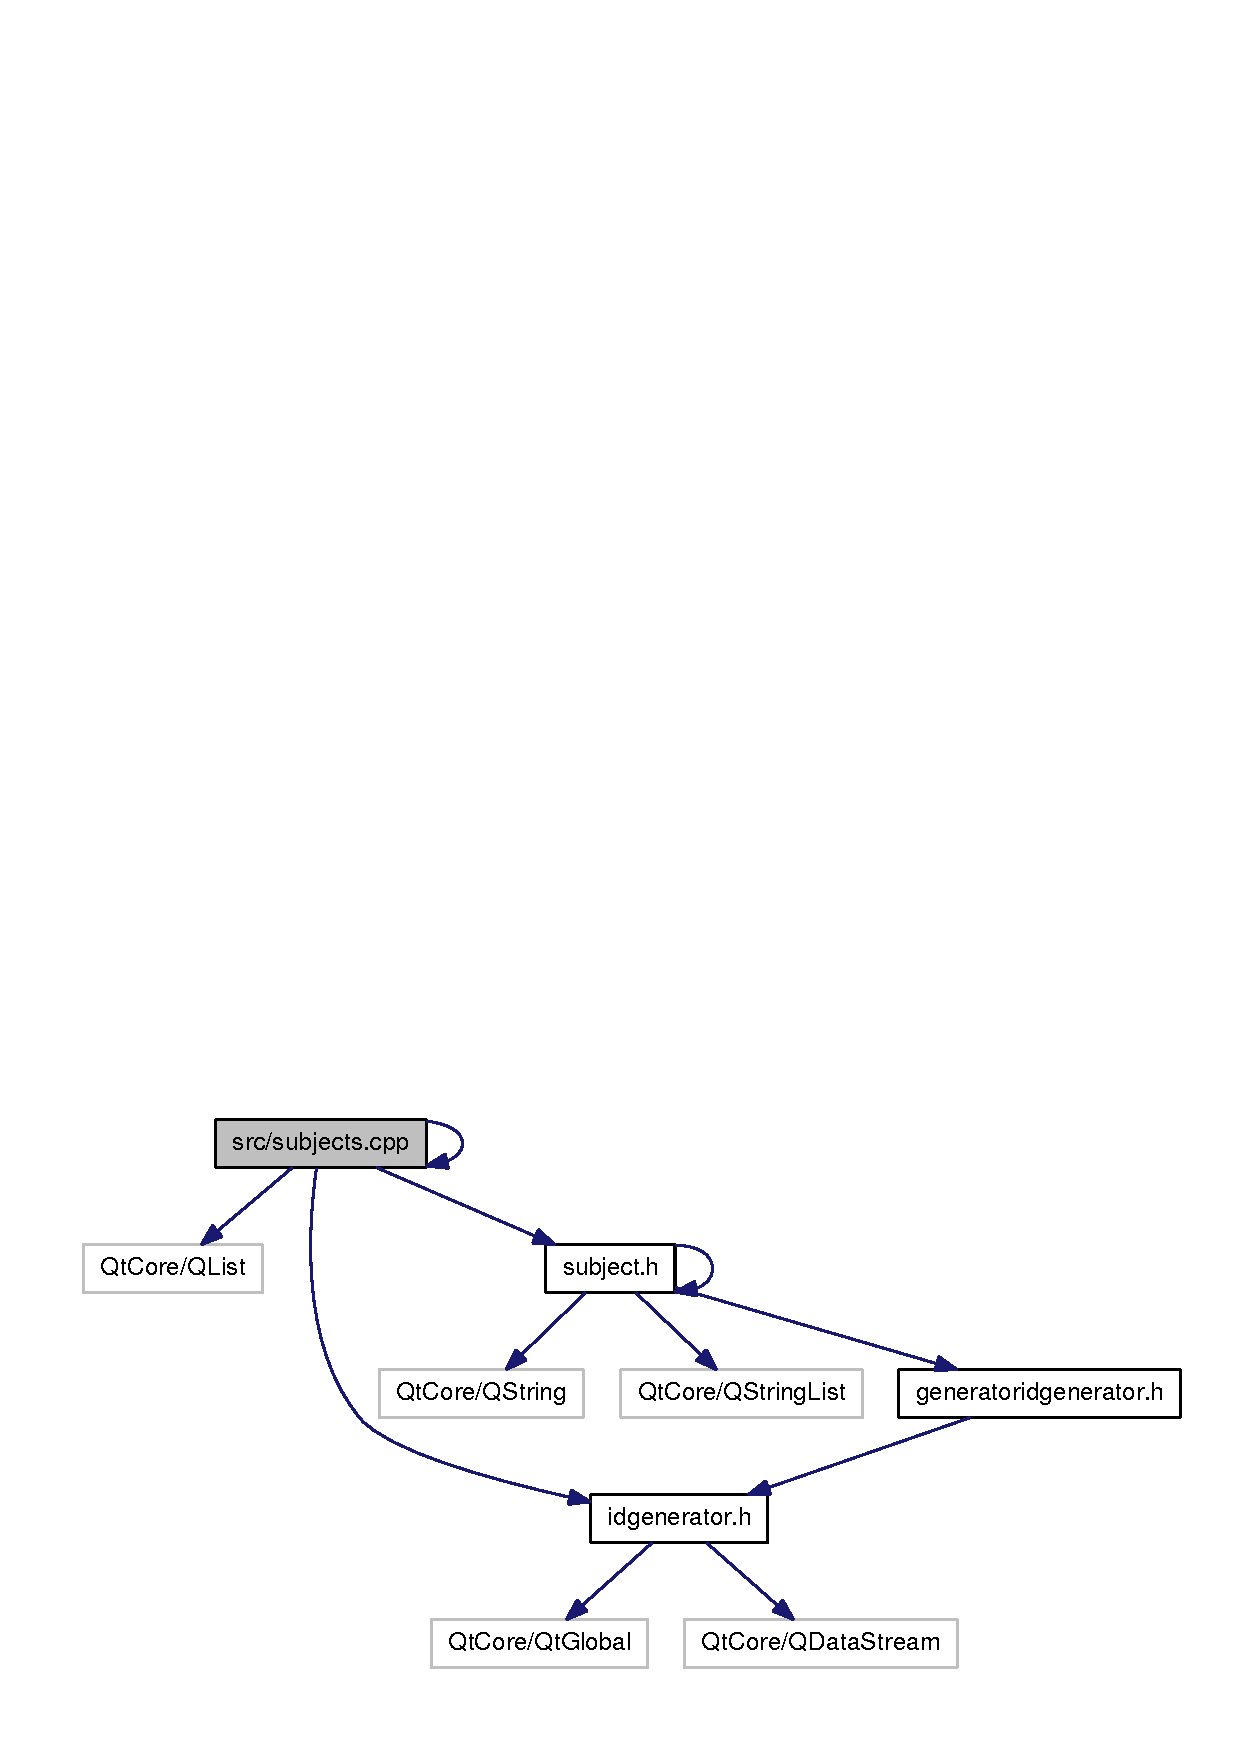
\includegraphics[width=285pt]{subjects_8cpp__incl}
\end{center}
\end{figure}
Ten wykres pokazuje, które pliki bezpośrednio lub pośrednio załączają ten plik:\nopagebreak
\begin{figure}[H]
\begin{center}
\leavevmode

\includegraphics[width=81pt]{subjects_8cpp__dep__incl}
\end{center}
\end{figure}
